\chapter{Problem statement}


The goal of super resolution (SR) is to produce a high resolution image from a low resolution input. Rather than simply interpolating the unknown pixel values we wish to infer their true value based on the information in the input. To do this we introduce the super resolution equation.

\begin{figure}[htb]
    \centering
    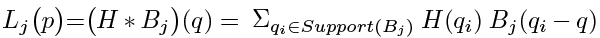
\includegraphics[width=\linewidth]{eq1.png}
    \caption{Super resolution}
    \label{fig:eq1} % insert suitable label, this is used to refer to a fig from within the text
\end{figure}


Where $Lj(p)$ denotes the value of the pixel at location p in the low resolution image. Similarly $H(q)$ denotes the value at pixel location q in the latent high resolution image. $B(.)$ is the blur kernel, or point spread function (PSF). The subscript j denotes a particular low-res image and blur kernel, which will be described later. Equation states that the low resolution image is assumed to be the result of a convolution between the high resolution image and a PSF and then down-sampled.

\begin{figure}[htb]
    \centering
    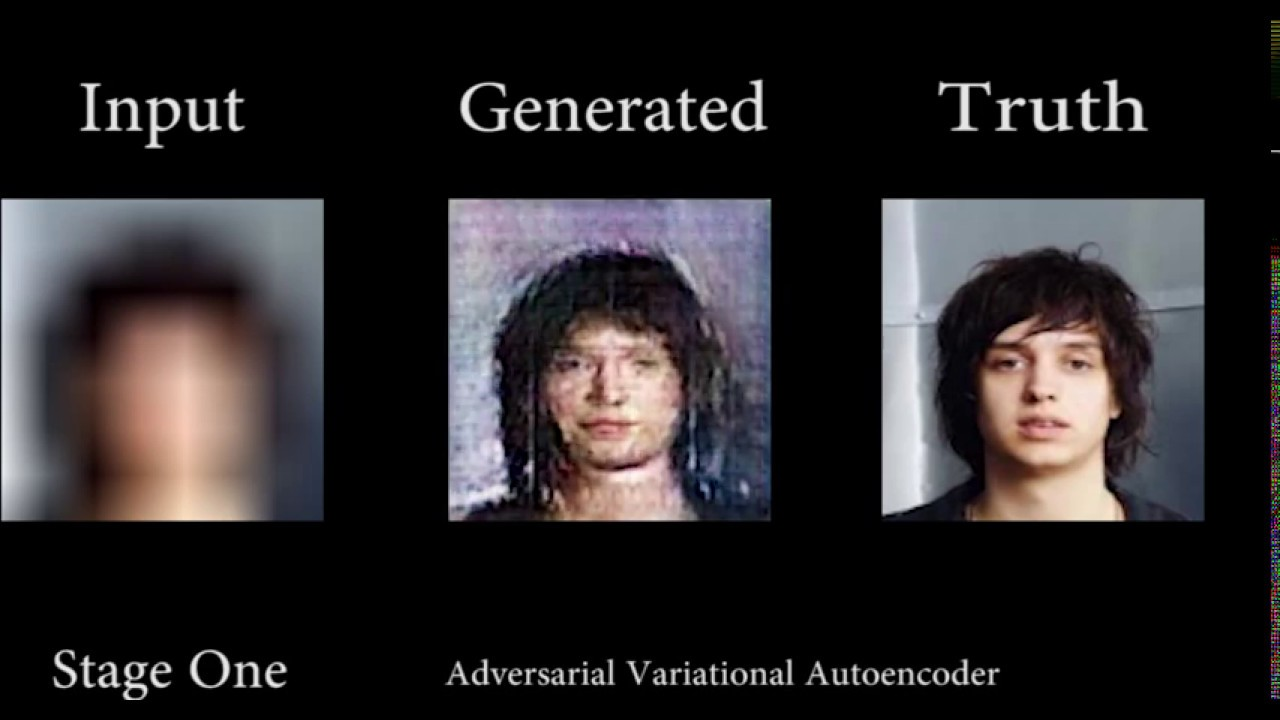
\includegraphics[width=\linewidth]{sr4.jpg}
    \caption{Better edge correction}
    \label{fig:sr4} % insert suitable label, this is used to refer to a fig from within the text
\end{figure}

Because convolution is a linear operation the above equation induces a set of linear constraints on the latent high resolution image H. Given only a single low resolution image, though, the equation is underconstrained.

Using the concept of patch redundancy it is possible to at least approximate a solution to the equation using only a single image. In D. Glasner, S. Bagon, M. Irani the authors present an algorithm for performing super resolution from a single image. This project implements the specified algorithm and presents results on a set of images.

